\section{Experimental procedure}
	\subsection{Making of the Kinesin-1-stepping assay}
	% TODO: describe making of the specimen; create graphic that visualises the purpose of the used chemicals
	
		
		We started the experiment with preparing the specimen that is visualised schematically in Figure \ref{exp:steppingAssay}. For that we got a hydrophobic object holder where the later mentioned antibodies and blocker-substances will bind to. Two flow channels were formed by placing 3 stripes made of paraffin on the slide that seal the channels under the coverslip after a short heating procedure. Then these channels were flooded by several chemicals. At first we filled in the \textit{BRB80} buffersolution. That is necessary to hold the pH-Value approximately constant. Then we put the \textit{Anti-$\beta$-tubulin antibodies} in the channel that bind the microtubules to the surface of the object holder. The experiment of our group unfortunately failed probably because of using a too thin antibody-solution in this step. For hindering proteins other than the microtubules to bind to the surface of the slide we now wash the channel with some blocker-substances: \textit{F127} and \textit{Casein}. Because microtubules are highly dynamic filaments we have to stabilise them somehow. For this purpose we combine our BRB buffersolution with \textit{taxol} that prevents the depolymerisation of tubulin. So finally we can put the rhodamine-labeled \textit{microtubules} and the \textit{kinesin-1 motorproteins} that are dyed with GFP in the channel. The kinesin-solution is enriched with \textit{MgATP} that is the 'fuel' of the motorpretein's-motion. Additionally a \textit{glucose-based antifade-cocktail} is used to surpress the reaction of free-radicals created by strongly excited fluorophores with free-oxygen of about a factor 2. This is necessary to reduce the photobleaching and the damaging of the proteins.
 		\begin{figure}[H]
 			\centering
 		   	\captionsetup{justification=raggedright, margin =4cm}            
 		    	  \includegraphics[scale=0.3]{pic/steppingassay.png}
 		    \caption{Schematic scetch of the stepping assay. 1-Hydrophobic slide, 2-Anti-$\beta$-tubulin antibody, 3-MT, 4-Taxol stabilisator, 5-motor-protein, 6-ATP - 'fuel', 7-block substances (F127, Casein)}
 		   	\label{exp:steppingAssay} 
 		\end{figure}
 		\ \\
 		Now we are ready for taking the movies of our stepping-assay.
    	     	                 
    	 

	\subsection{Stream acquisition}
        First the experimental supervisor placed the flow cell holder on the microscope stage. We used an oil objective which has to touch the bottom of the flow cell. The objective has a magnification of 100x and a numerical aperture of $1.46$.  
        After the assay was fixed we used a Software called MetaMorph. We used a digital Camera by Andor which took greyscaled pictures. Its resolution is $\unit[2.6]{MPixel}$ with 512x512 pixels. The size of one pixel ist $\unit[25600]{nm^2}$.
        According to the meta data of the movies and pictures the chosen additional magnification of the camera is 1.0x. This means, the pixel size is the original pixel size of the camera. If it had been 2.5x, we could have seen 2.5 times less, so a pixel would have been $A = \unit[25600]{nm^2} / 2.5 = 10240\ \unit{nm^2}$. 
        So we took the TRITC filter and the lamp on the taskbar and watched the live images token by the camera. We searched and focused a cutout where we could see enough MTs. 
        Unfortunately our assay showed that no MT's were fixed in it, so we could not take any pictures. Maybe this was caused by a too thin microtubule- or antibody-solution. We used the assay of our co-workers instead.\\ 
        After we focused the MTs, we stopped live imaging and took pictures of the MTs luminescated by rhodamine. After that we take the GFP filter and choose the laser illumination. Then we choose again live imaging ("show live"). The TIRF angle will be adjusted.  %note: can we make out the transiotion to the tirf mode?
        Again we choose the TRITC filter on the taskbar, the lamp illumination and take live imaging. We move to a new field of view, focus properly and take an image of the MTs such as in figure \ref{exp:mts}.\\
        \begin{center}
             \includegraphics[scale=0.4]{pic/exampleMT.jpeg}  
             \captionof{figure}{Example of an image, where we focused on the MTs}
             \label{exp:mts}
        \end{center}
        Then we save an image of this position. We now switched again to the GFP filter, selected the laser as light source and take live imaging. We can see moving motors. We stop live imaging and take a movie via the acquire button. The number of frames we took is 1000. 
        For one frame the camera needs $\unit[150]{ms}$, so at the end one we wait 150s per video stream. We took 8 movies. 
        When all streams are collected, one can do the data processing with FIESTA. There you can mark the possible trajectories of the motor proteins (as seen in figure \ref{exp:markex1}) and the software will calculate pieces of the picture where the height is the time dimension and the width is the movement. If there is motion, one can mark up the lines and get the time which was needed for the marked distance (see figure \ref{exp:markex2}).
        \begin{center}
                \begin{tabular}{p{7cm}p{5cm}c}
                   \minipanf 
                        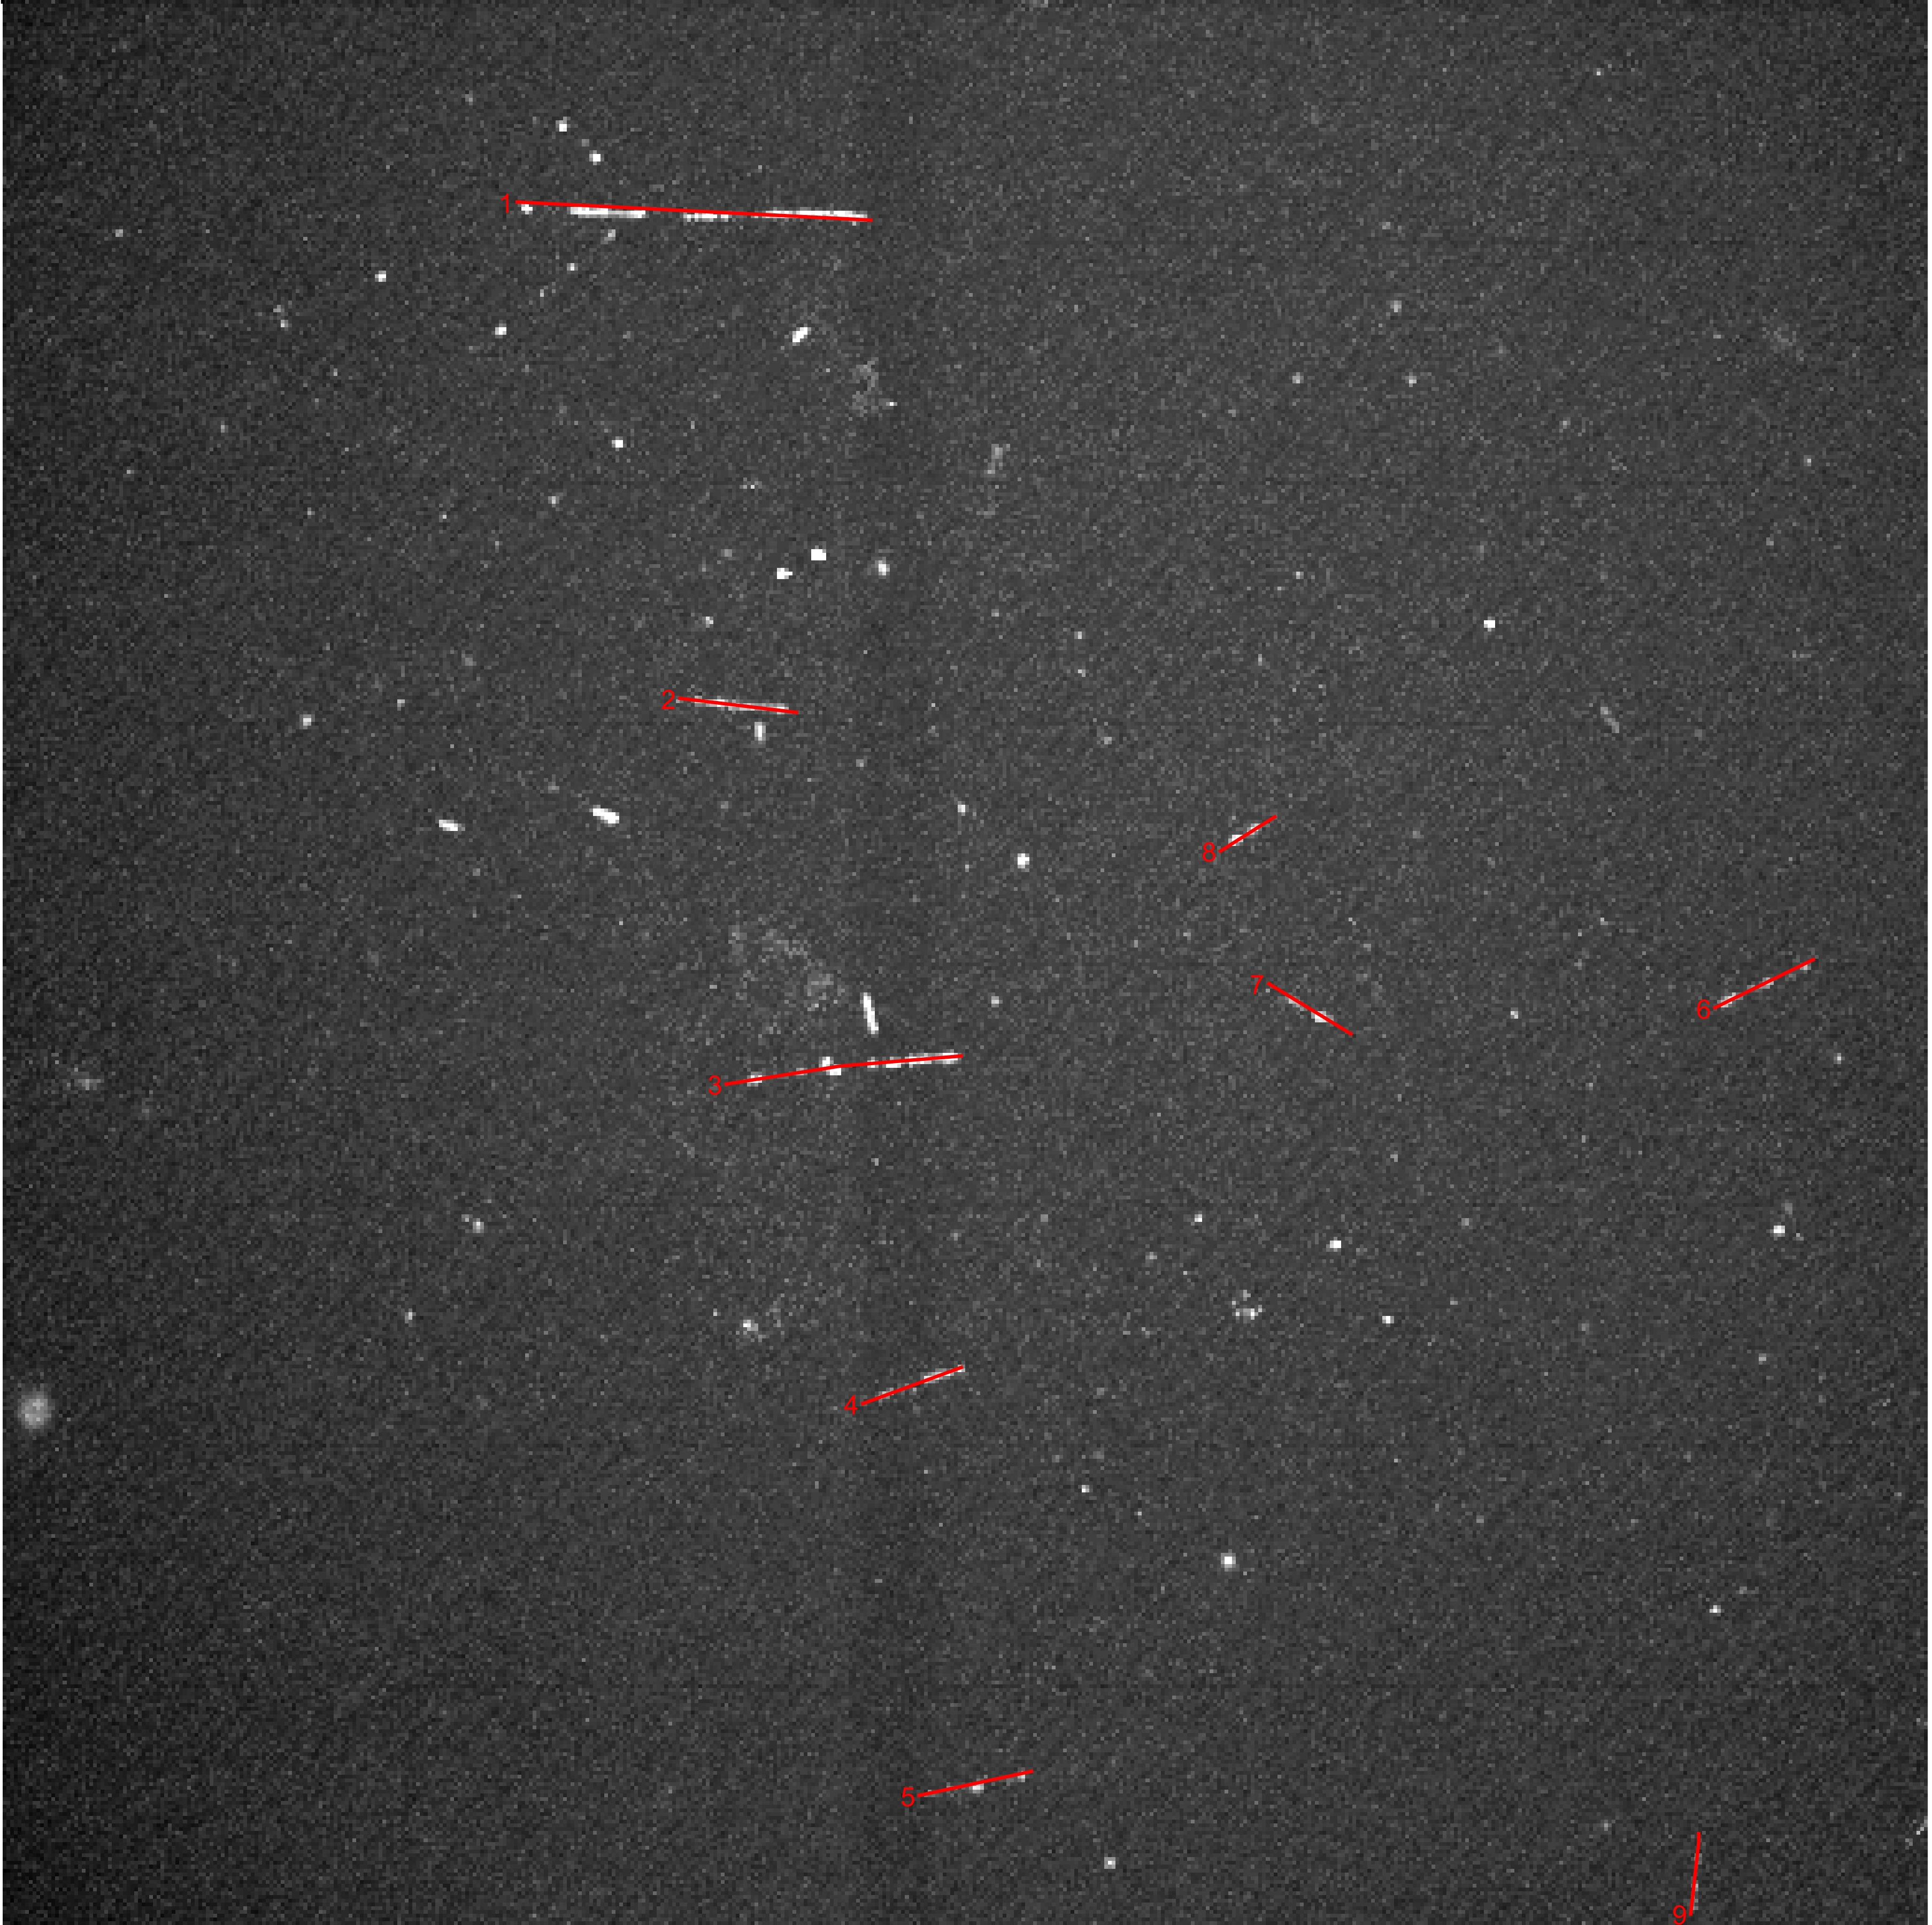
\includegraphics[scale=0.05]{pic/example_marked_tubules.jpg}
                        \captionof{figure}{first step marking of the microtubules}
                        \label{exp:markex1}
                   \minipend 
                   &
                   \minipanf
                     \begin{center}
                       \includegraphics[scale=0.0333]{pic/example_distances_time_marked.jpg}
                       \captionof{figure}{marking of the trajectories of the motor proteins}
                       \label{exp:markex2}
                     \end{center}
                   \minipend
                \end{tabular}    
        \end{center}
